% --- DeepSeek-R1 Case Study ---
\begin{frame}{Example of Reinforcement Learning for Reasoning Skill Refinement: DeepSeek-R1}
  \centering
  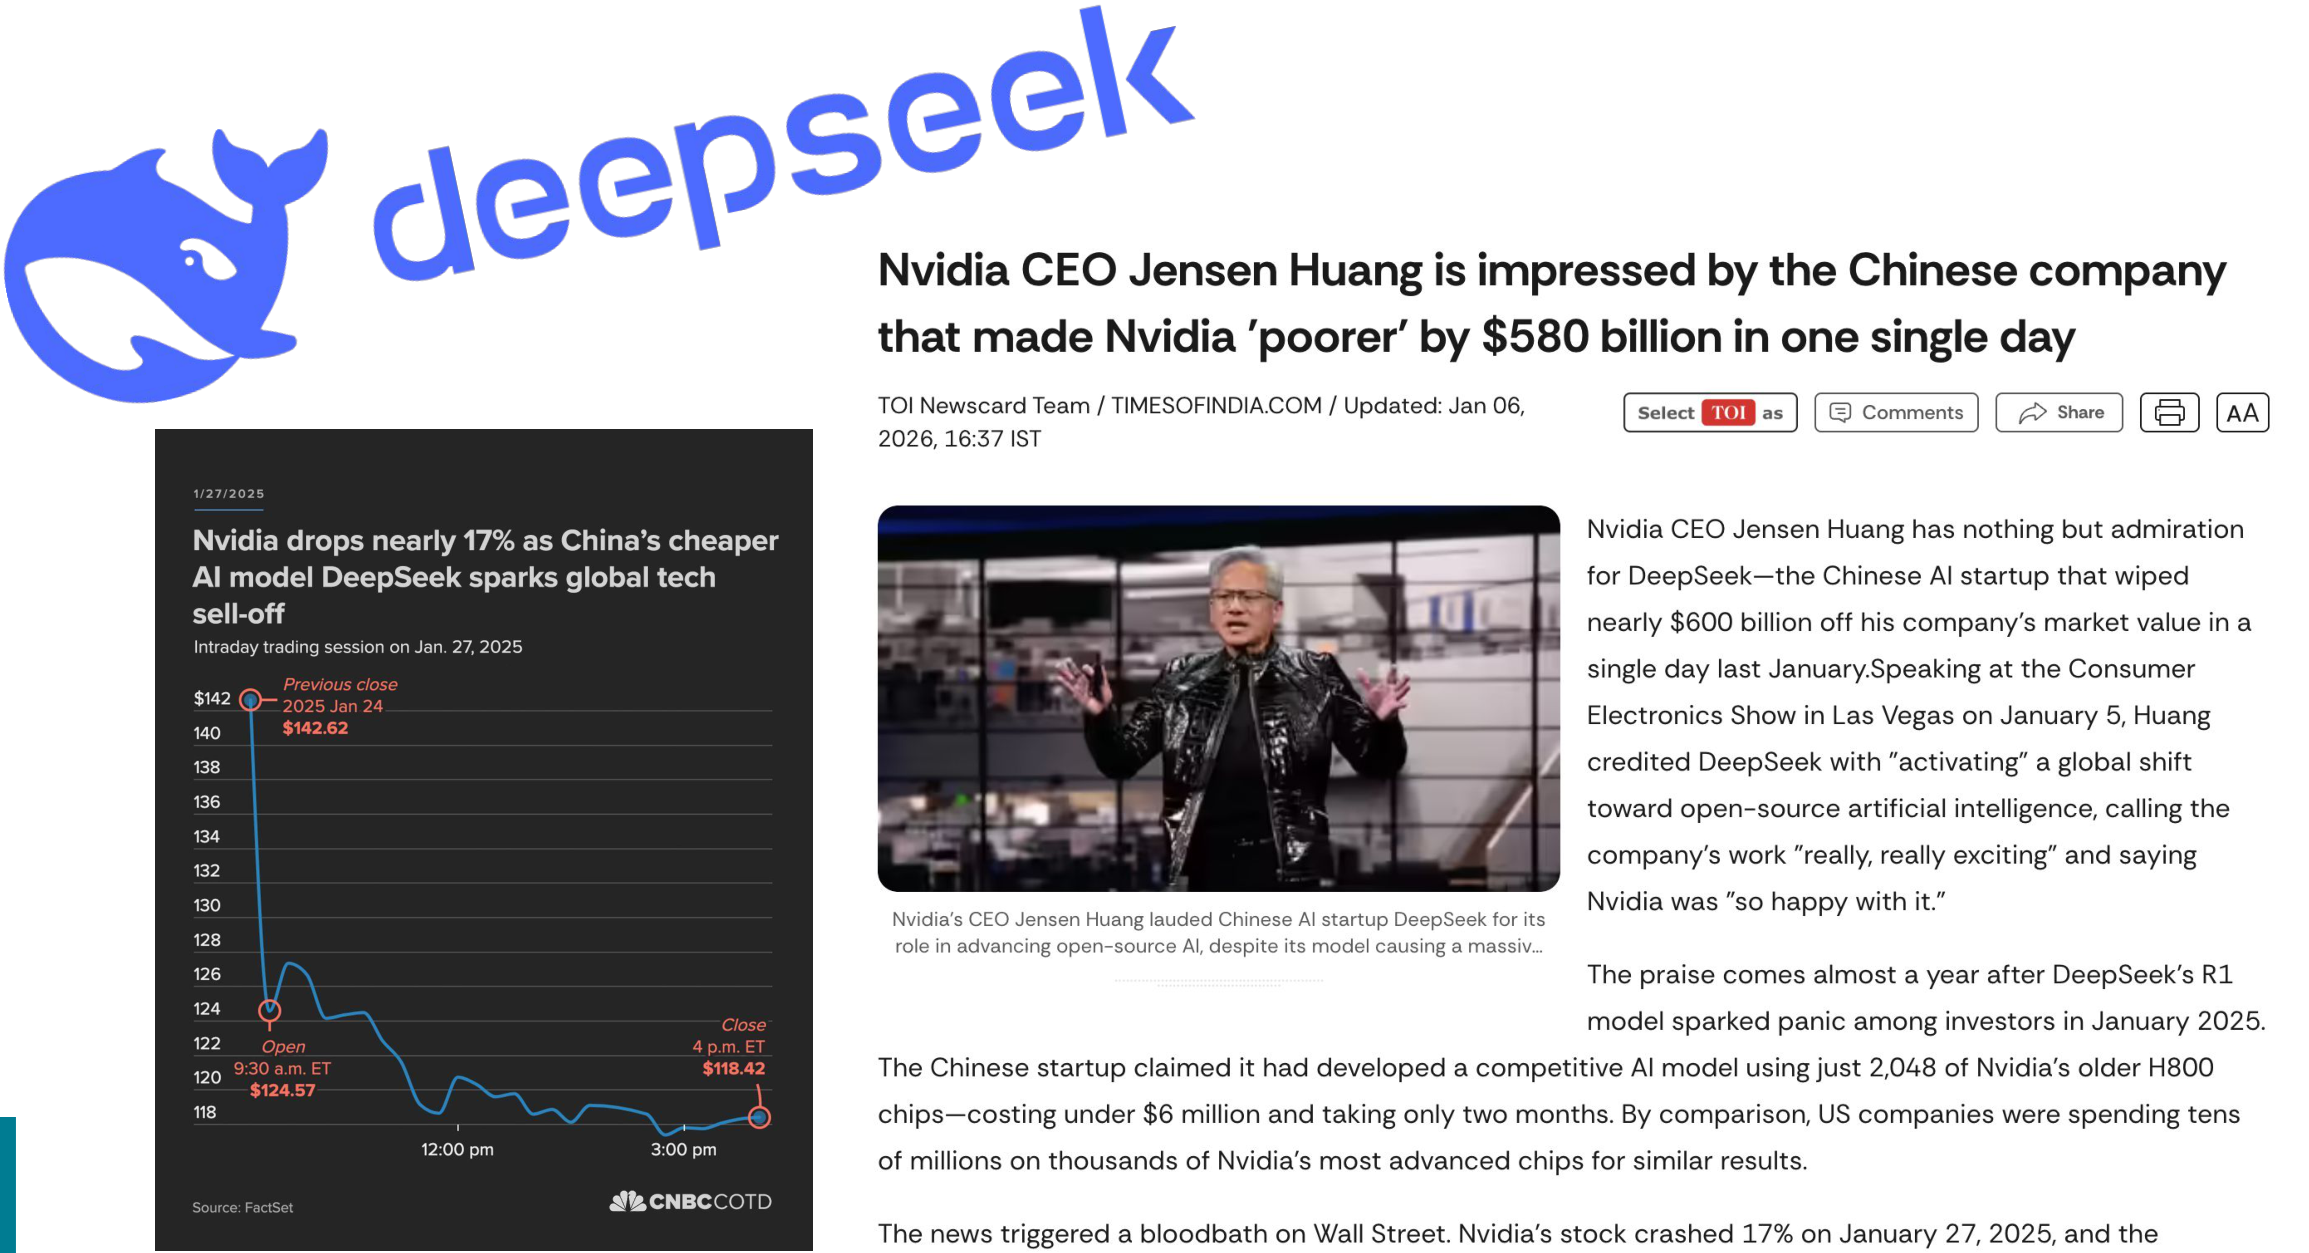
\includegraphics[width=\textwidth,height=0.90\textheight,keepaspectratio]{assets/New-Lecture-LRM/cs224n_2026_lec12_p23_deepseek.png}
\end{frame}

\begin{frame}{Example of Reinforcement Learning for Reasoning Skill Refinement: DeepSeek-R1}
  \begin{figure}
    \centering
    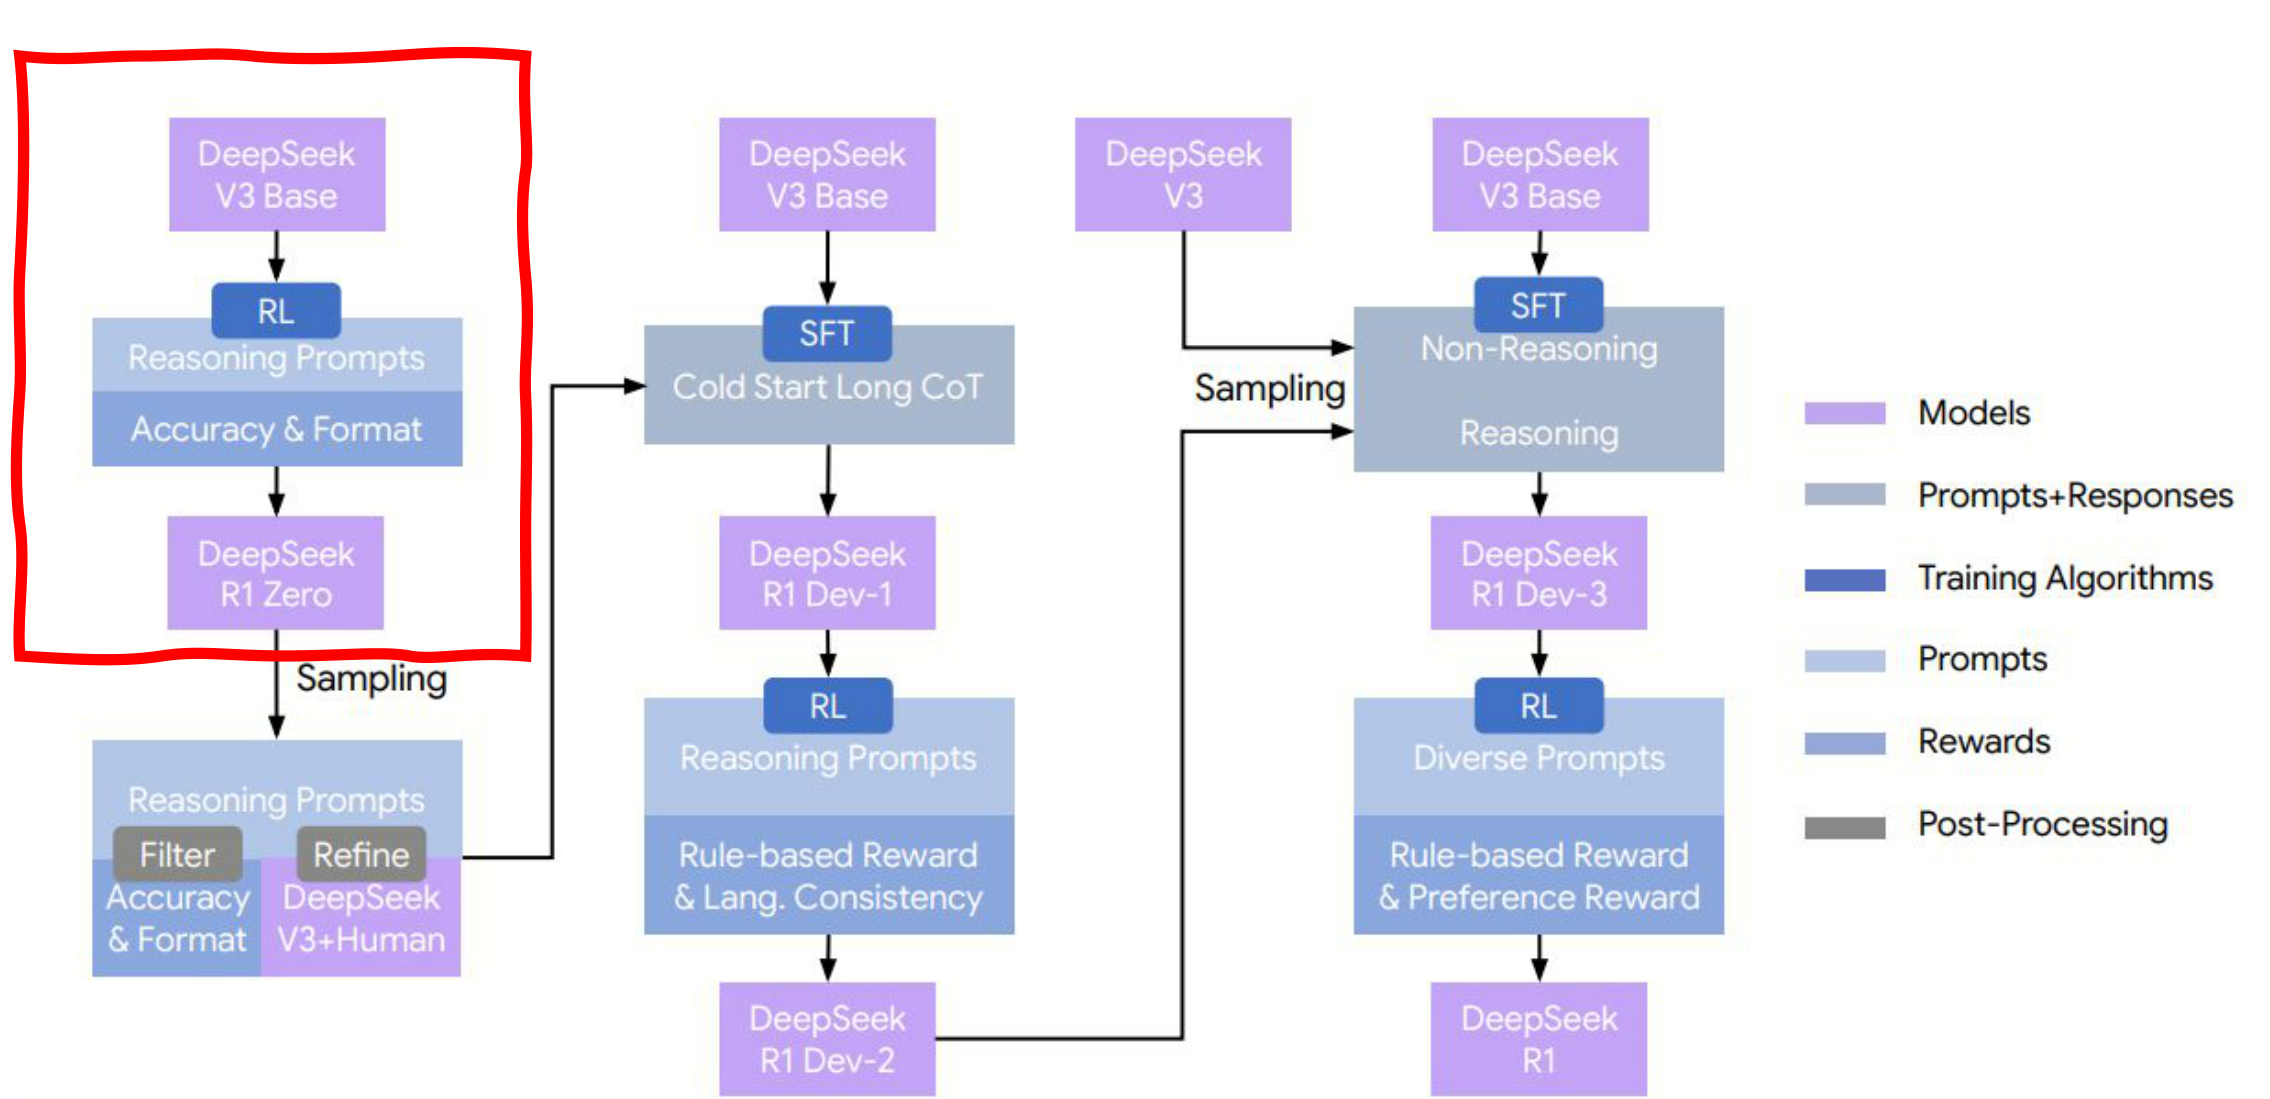
\includegraphics[width=\textwidth,height=0.90\textheight,keepaspectratio]{assets/New-Lecture-LRM/cs224n_2026_lec12_p24_deepseek.png}
    \caption*{DeepSeek-R1 training pipeline overview. Source: Choi (2026) \href{https://arxiv.org/abs/2501.12948}{arXiv:2501.12948}.}
  \end{figure}
\end{frame}

\begin{frame}{Example of Reinforcement Learning for Reasoning Skill Refinement: DeepSeek-R1}
  \begin{figure}
    \centering
    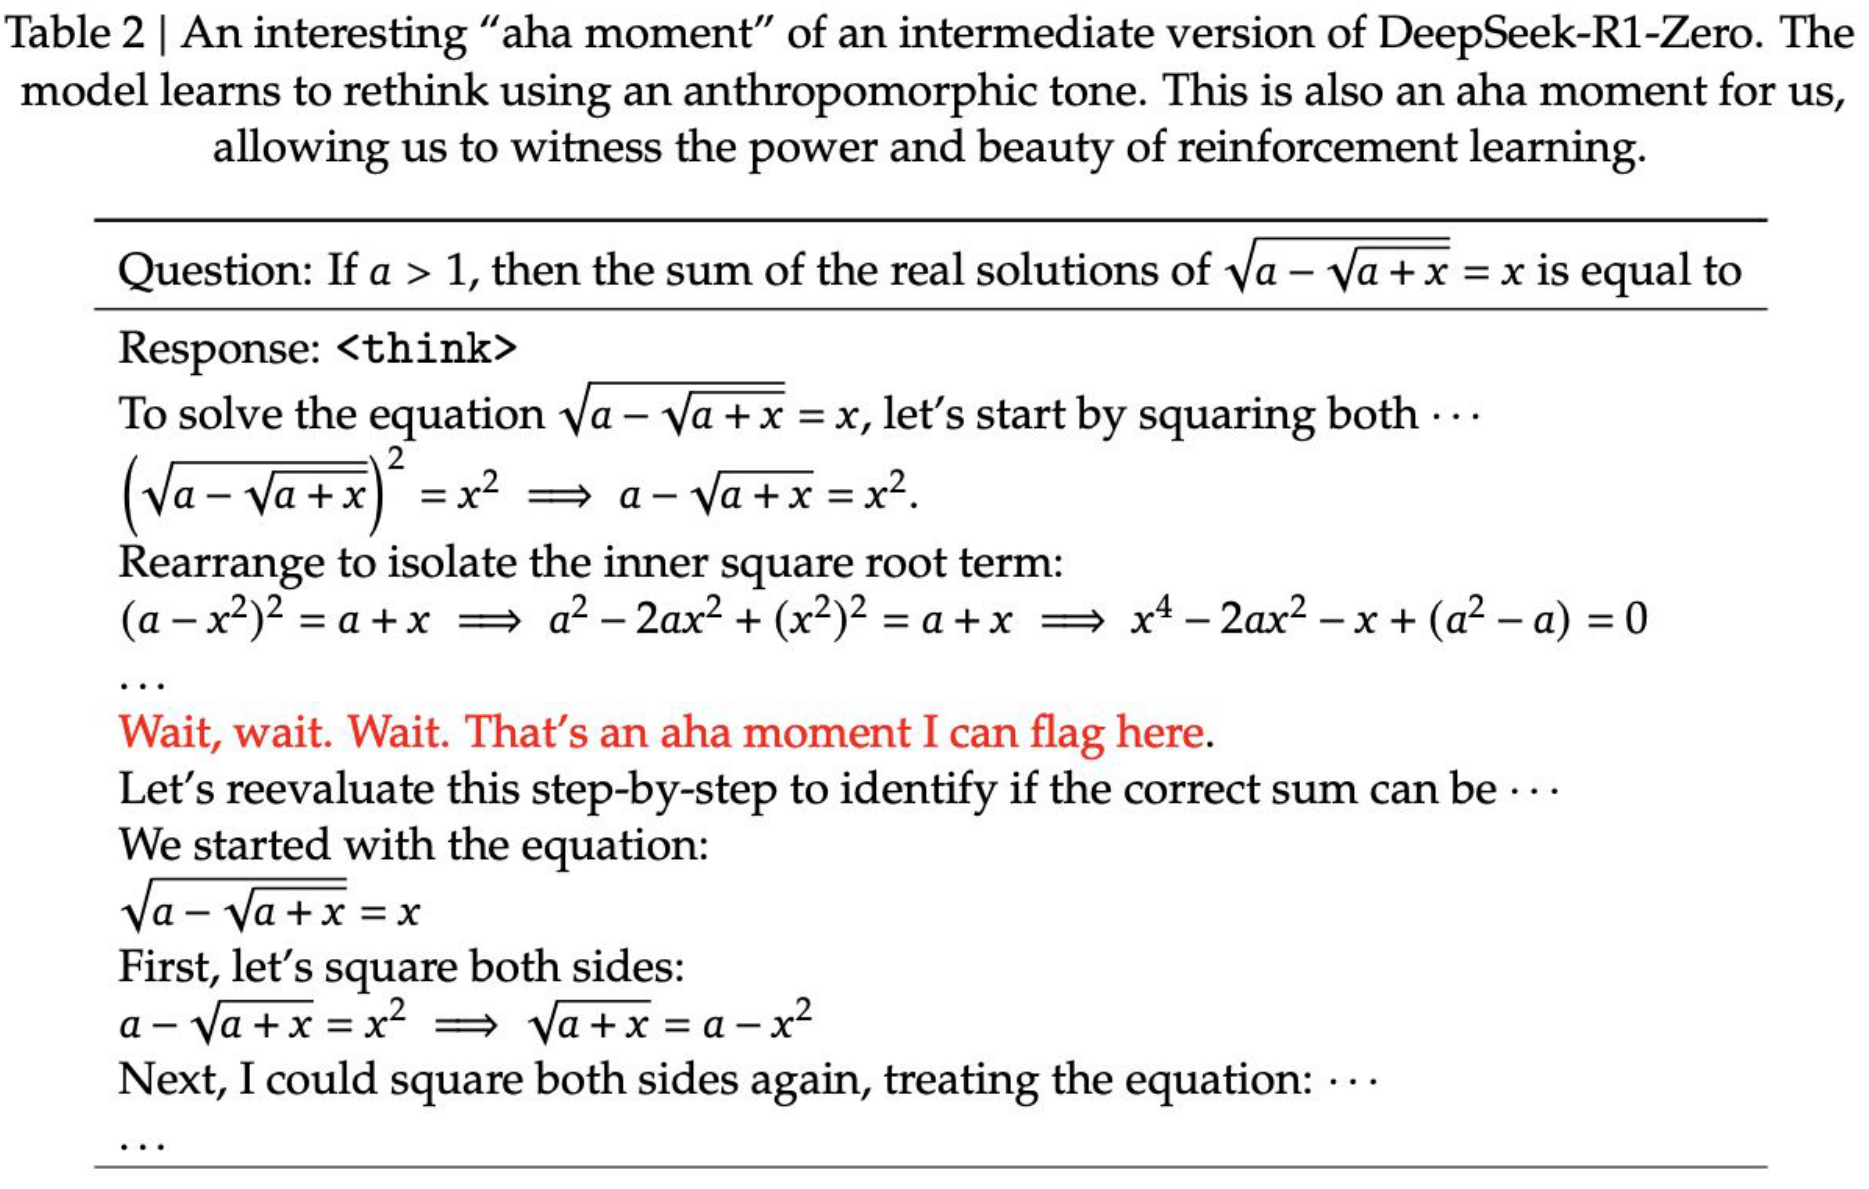
\includegraphics[width=\textwidth,height=0.90\textheight,keepaspectratio]{assets/New-Lecture-LRM/cs224n_2026_lec12_p25_deepseek.png}
  \end{figure}
\end{frame}

\begin{frame}{Reward for R1-zero: keeping it simple}
    \centering
    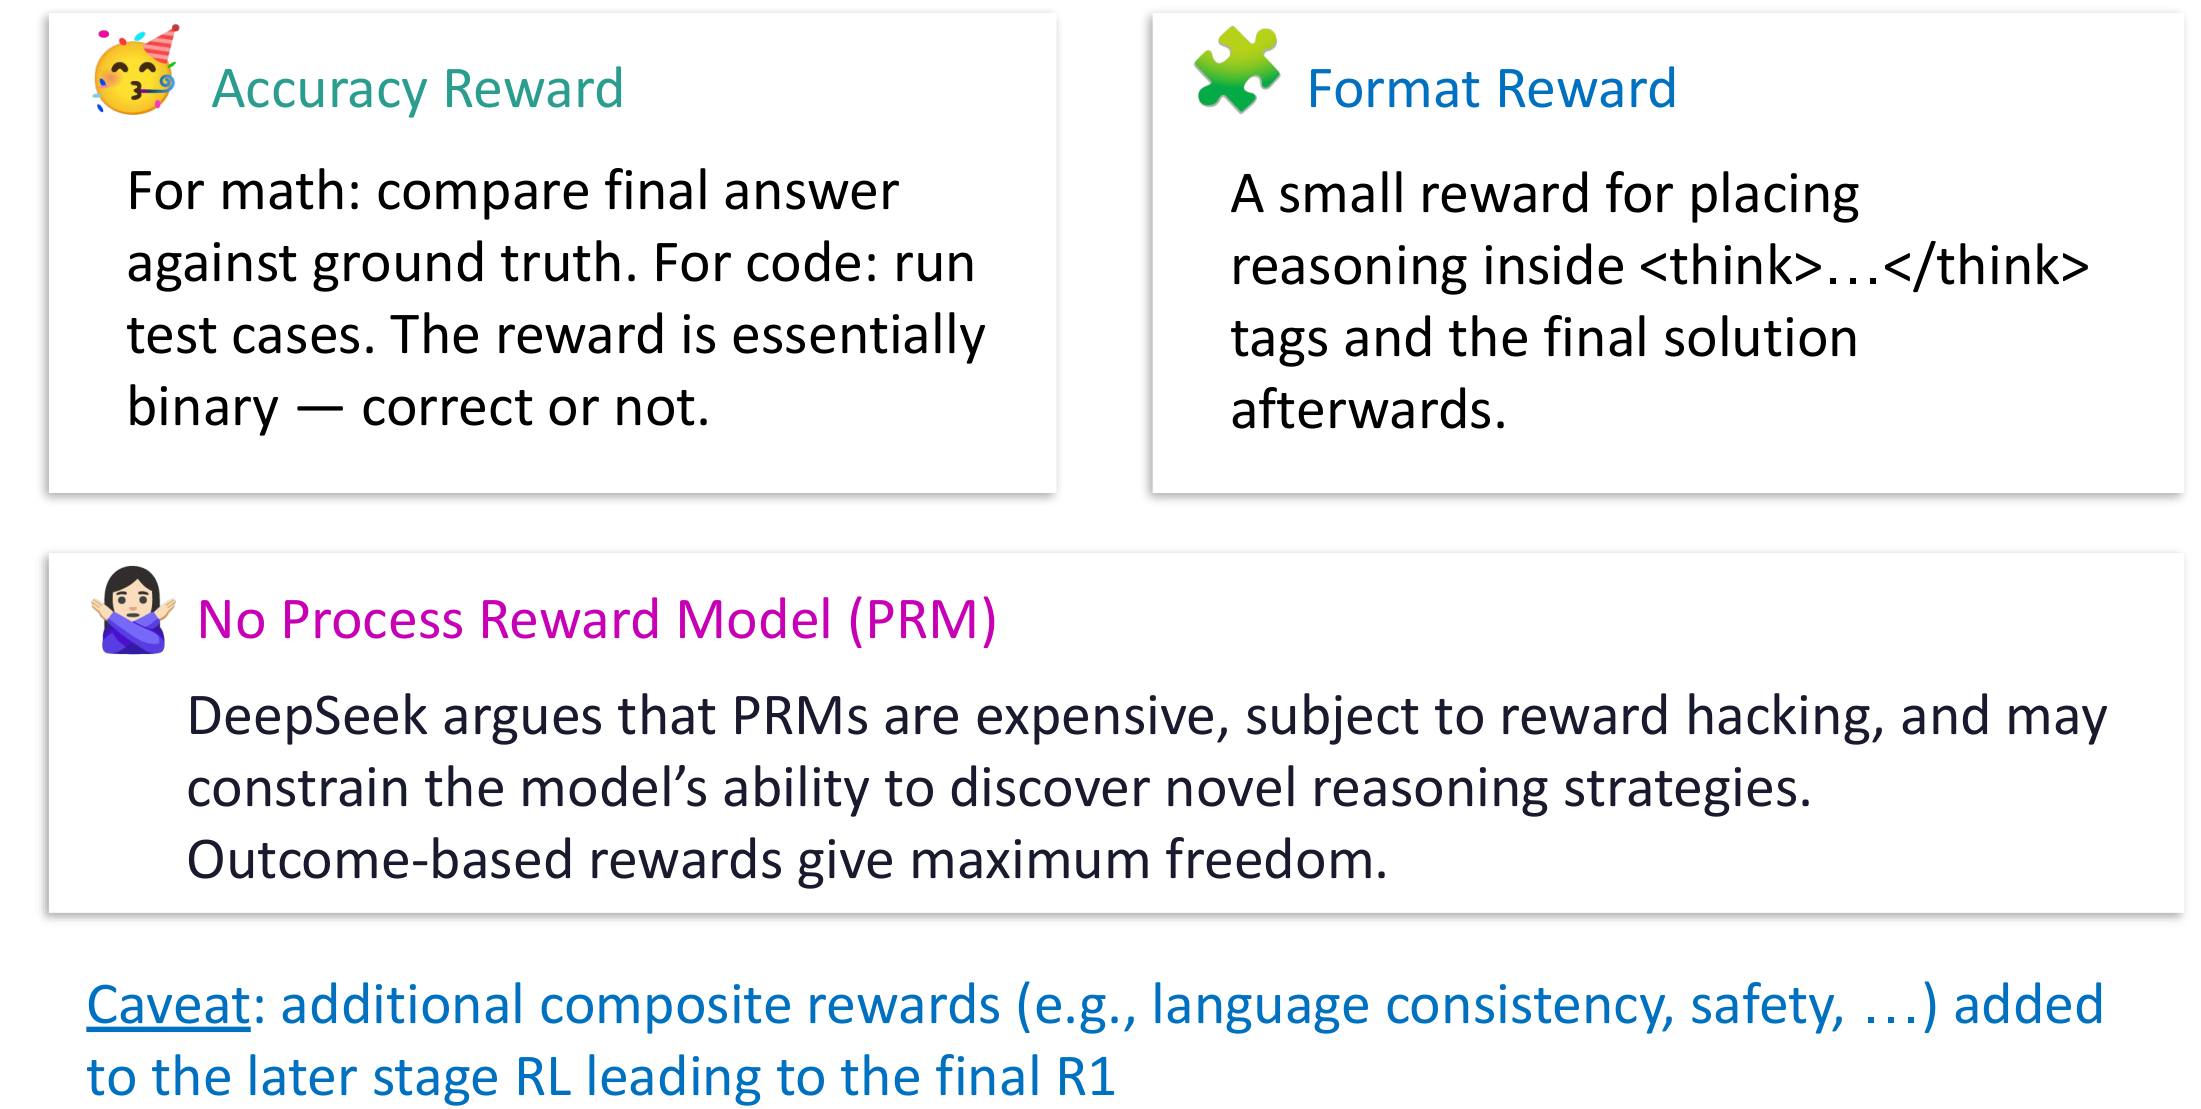
\includegraphics[width=\textwidth,height=0.90\textheight,keepaspectratio]{assets/New-Lecture-LRM/cs224n_2026_lec12_p26_deepseek.png}
\end{frame}

\begin{frame}{Emergent reasoning capabilities}
  \begin{figure}
    \centering
    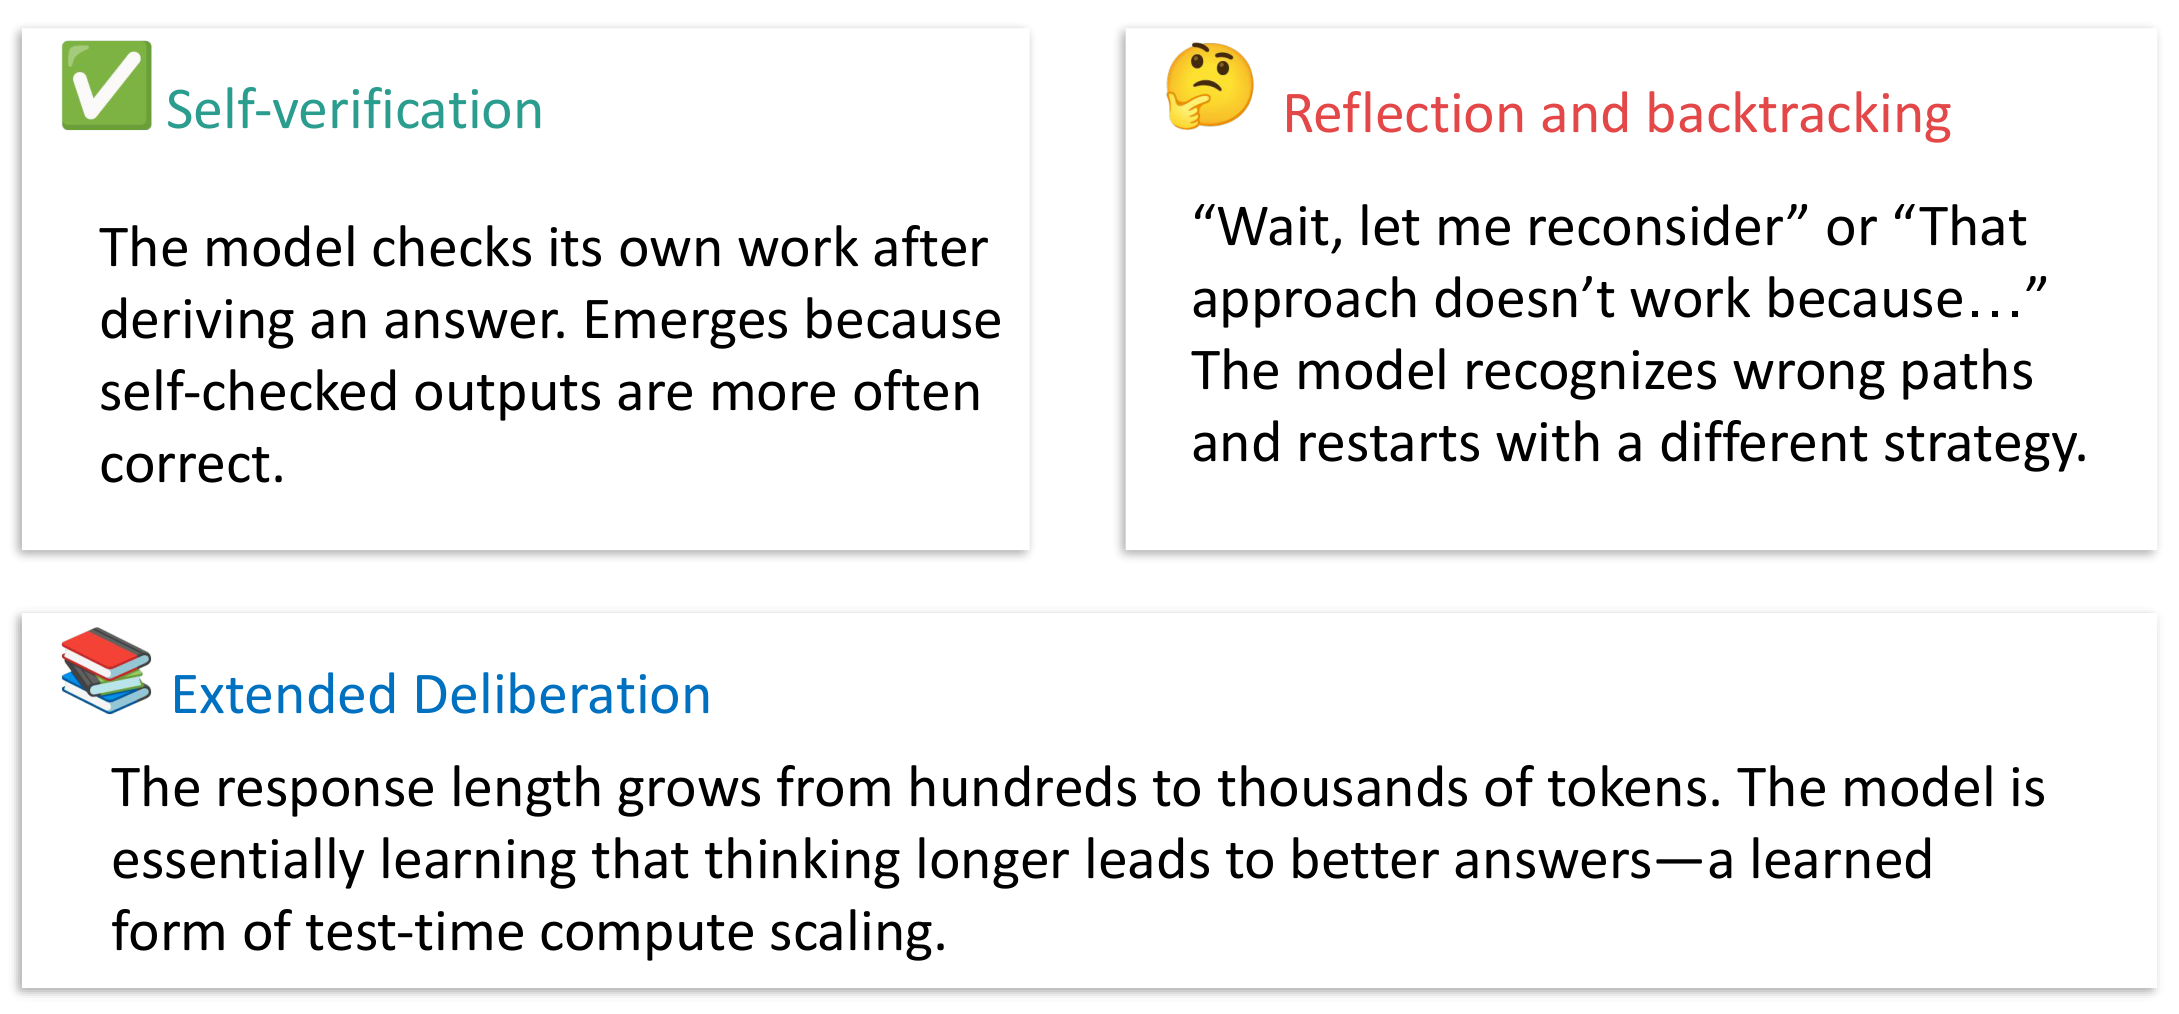
\includegraphics[width=\textwidth,height=0.90\textheight,keepaspectratio]{assets/New-Lecture-LRM/cs224n_2026_lec12_p27_deepseek.png}
  \end{figure}
\end{frame}

\begin{frame}{Emergent undesirable characteristics of R1-Zero}
  \begin{figure}
    \centering
    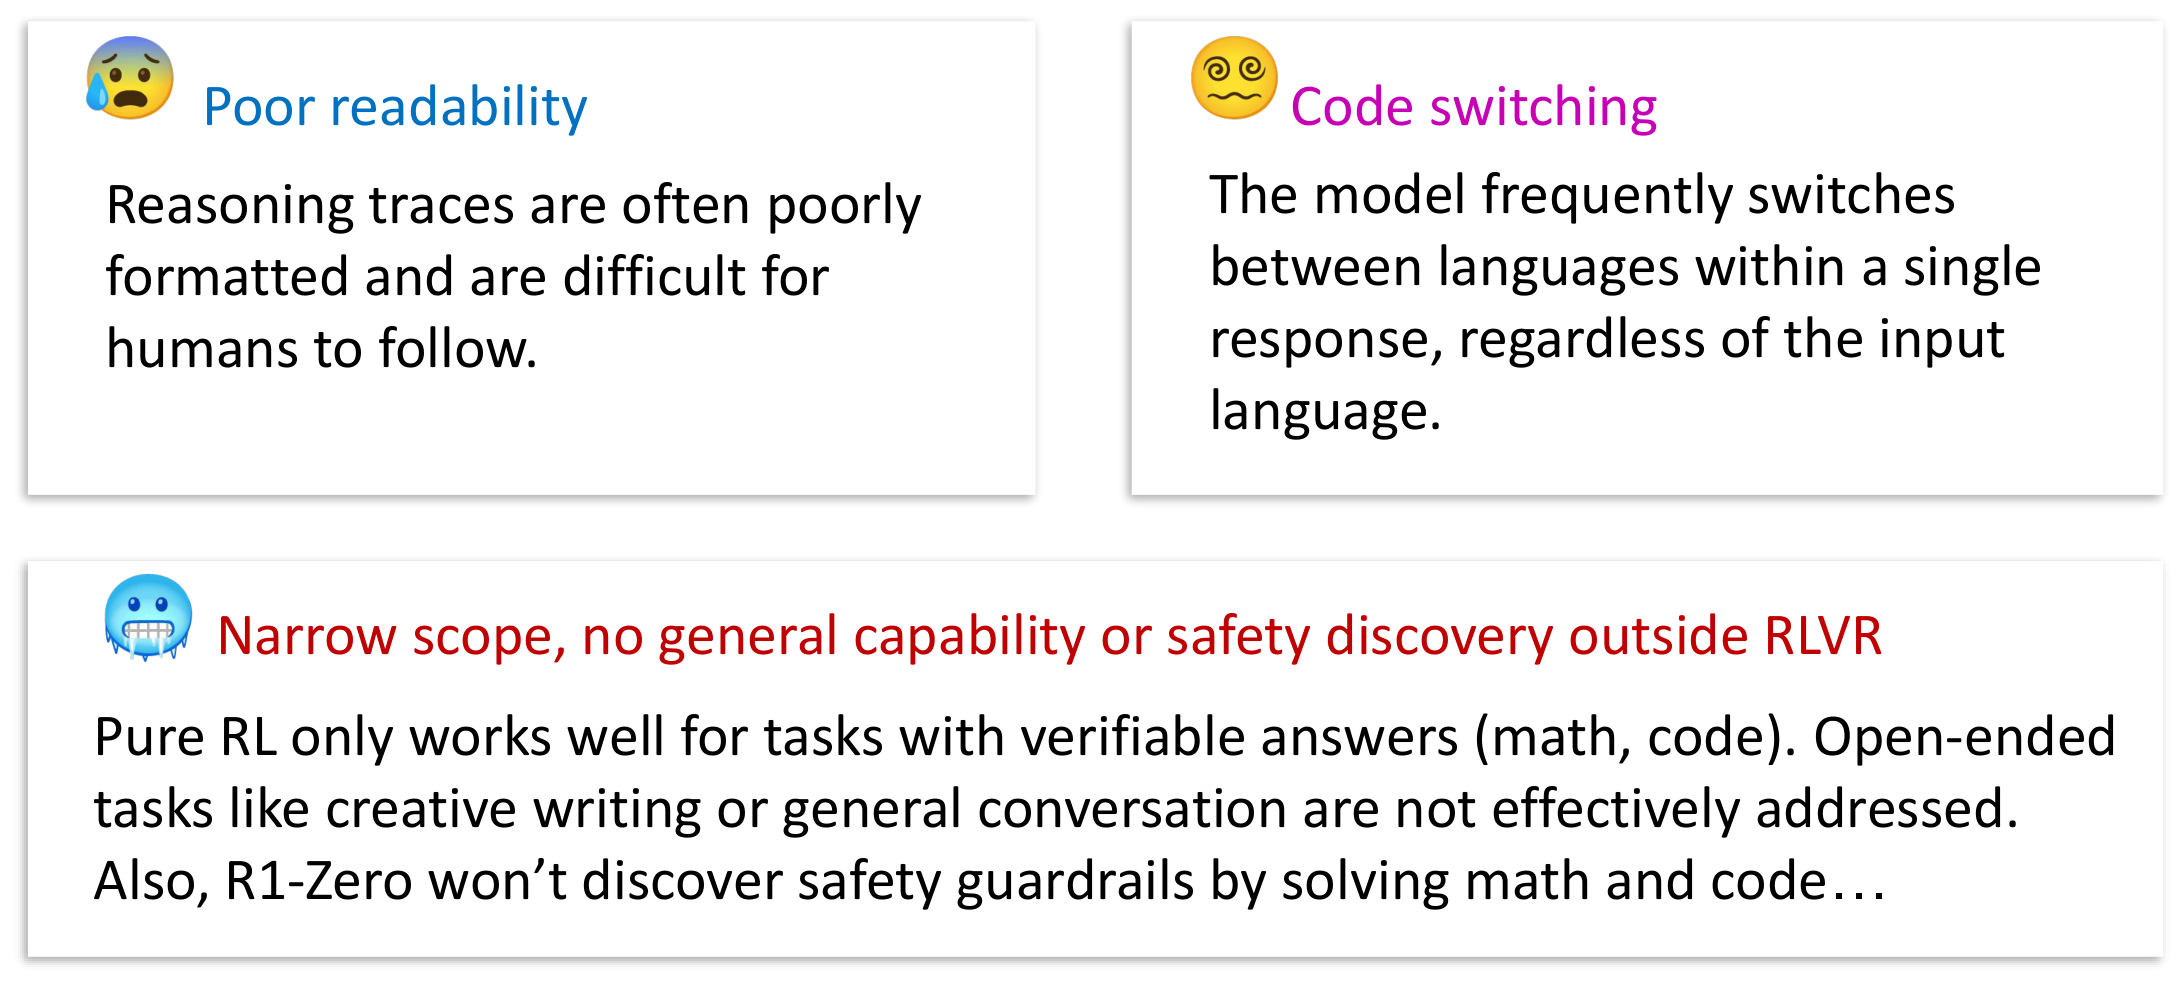
\includegraphics[width=\textwidth,height=0.90\textheight,keepaspectratio]{assets/New-Lecture-LRM/cs224n_2026_lec12_p28_deepseek.png}
  \end{figure}
\end{frame}

\begin{frame}{Example of Reinforcement Learning for Reasoning Skill Refinement: DeepSeek-R1}
  \begin{figure}
    \centering
    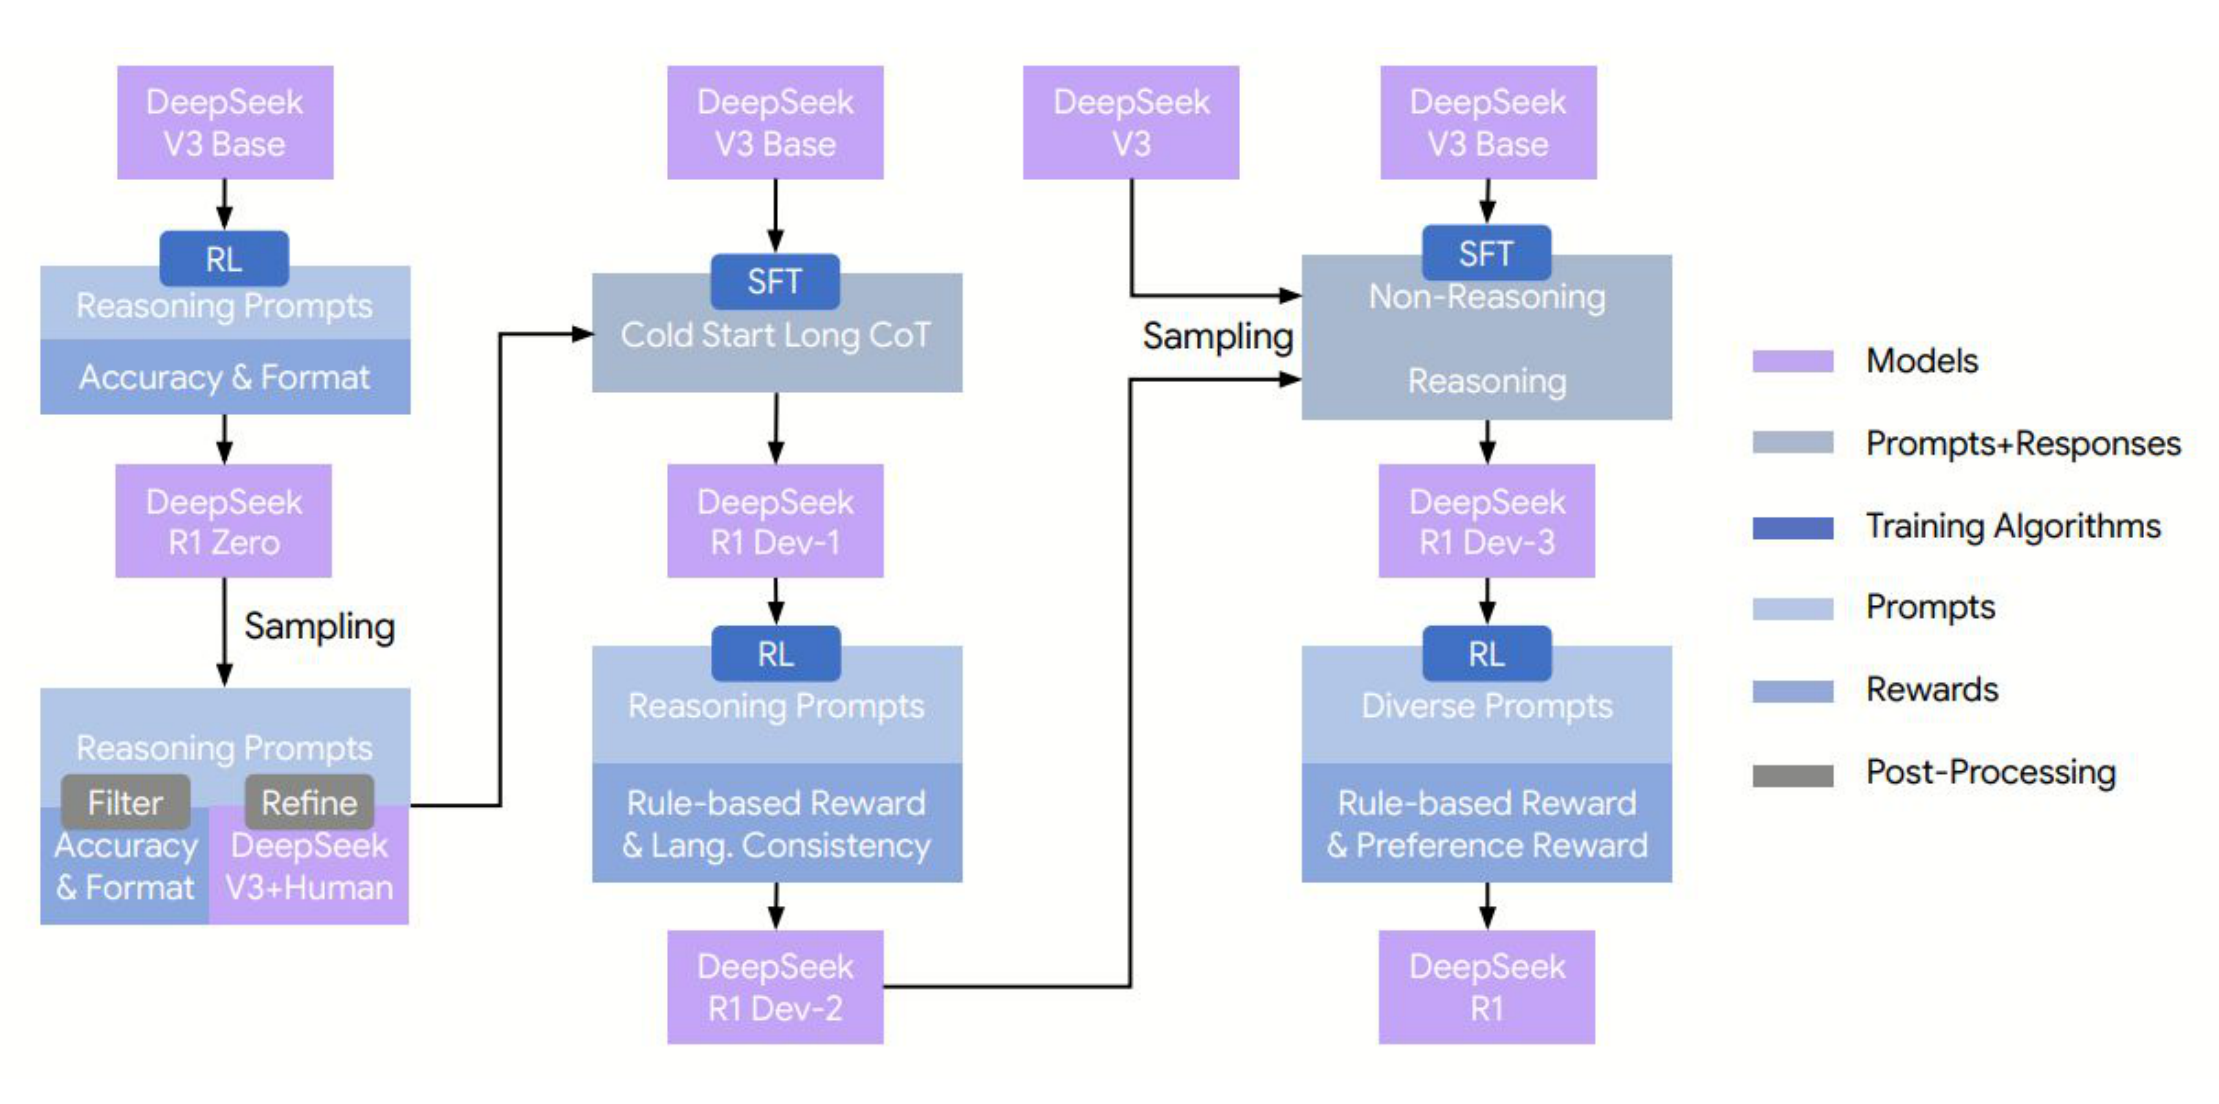
\includegraphics[width=\textwidth,height=0.90\textheight,keepaspectratio]{assets/New-Lecture-LRM/cs224n_2026_lec12_p29_deepseek.png}
  \end{figure}
\end{frame}

\begin{frame}{Key findings: DeepSeek-R1}
  \begin{itemize}
    \item<1-> \textcolor{KAred}{\textbf{Finding 1: RL alone can induce reasoning}}
    \begin{itemize}
      \item \textbf{Prior assumption}: chain-of-thought reasoning required supervised examples.
      \item \textbf{Finding}: R1-Zero demonstrates that outcome-based RL, with no process supervision, can induce sophisticated reasoning capabilities.
      \item \textbf{Caveat 1}: the final R1 is still going through the SFT$\rightarrow$RL pipeline in the end
      \item \textbf{Caveat 2}: doesn't apply to small (less capable) models
    \end{itemize}
  \end{itemize}
\end{frame}

\begin{frame}{Key findings: DeepSeek-R1}
  \begin{itemize}
    \item<1-> \textcolor{KAred}{\textbf{Finding 2: Outcome rewards can enable discovery}}
    \begin{itemize}
      \item \textbf{Prior assumption}: sophisticated process rewards are necessary for O1 reasoning.
      \item \textbf{Finding}: Process reward models can inadvertently constrain exploration by penalizing unconventional yet effective reasoning paths. The lesson: sometimes less supervision yields more capability.
      \item \textbf{Caveat}: RLVR is not applicable for all reasoning problems.
    \end{itemize}
  \end{itemize}
\end{frame}

\begin{frame}{Key findings: DeepSeek-R1}
  \begin{itemize}
    \item<1-> \textcolor{KAred}{\textbf{Finding 3: RL + SFT synergy}}
    \begin{itemize}
      \item Neither pure RL (R1-Zero) nor pure SFT produces the best results.
      \item The multi-stage pipeline shows that RL and SFT play complementary roles: RL discovers capability, SFT provides reliability.
      \item Cold-start data prevents early RL instability; rejection sampling converts RL discoveries into reusable training data.
    \end{itemize}
  \end{itemize}
\end{frame}

\begin{frame}{Key findings: DeepSeek-R1}
  \begin{itemize}
    \item<1-> \textcolor{KAred}{\textbf{Finding 4: Distillation outperforms direct RL on small models}}
    \begin{itemize}
      \item If you have a limited compute budget, you are better off distilling from a large reasoning model than applying RL to a small model directly.
      \item Through distillation, reasoning capabilities transfer to models as small as 1.5B parameters, making strong reasoning accessible at any scale.
    \end{itemize}
    \item<2-> \textcolor{KAred}{\textbf{Finding 5: Open-weight reasoning models are viable}}
    \begin{itemize}
      \item R1 models are released under an MIT license.
      \item The distilled 7B and 14B models outperform many much larger closed-source models on reasoning benchmarks.
    \end{itemize}
  \end{itemize}
\end{frame}

\begin{frame}{Key findings}
  \begin{itemize}
    \item<1-> \textcolor{KAred}{\textbf{Finding 6: Structured search algorithms for inference scaling?}}\\
      \vspace{0.3em}
      \begin{itemize}
        \item \textbf{Prior assumption}: Inference-time search algorithm such as Monte-Carlo Tree Search might be necessary.
        \item \textbf{Findings}: Reasoning can be entirely autoregressive; no special search algorithm necessary.
        \item \textbf{Caveat}: Later models for hard math benchmarks do incorporate structure, though not in the traditional MCTS sense.
      \end{itemize}
  \end{itemize}
\end{frame}

\begin{frame}{Key findings: DeepSeek-R1}
  \begin{itemize}
    \item<1-> \textcolor{KAred}{\textbf{Finding 7: Test-time compute is a learnable resource}}
    \begin{itemize}
      \item \textbf{Findings}: R1’s models learn to allocate more thinking tokens to harder problems. This means test-time compute scaling is not just an inference trick (like beam search or majority voting)—it can be internalized by the model itself through training. The model learns when and how much to think.
      \item \textbf{Caveat}: true to some degree; later studies reveal challenges to address.
    \end{itemize}
  \end{itemize}
\end{frame}
